\documentclass[12pt]{beamer}

% INCLUDE GRAPHICS
\usepackage{graphicx}

% TABLES
\newcommand{\ra}[1]{\renewcommand{\arraystretch}{#1}} % spaces in tables
\usepackage{booktabs}   % Allows the use of \toprule, \midrule and \bottomrule in tables for horizontal lines

% FONTS
% PdfLatex
% \usepackage[T1]{fontenc}
% \usepackage{pgf}
% \logo{\pgfputat{\pgfxy(-1,-0.435)}{\pgfbox[center,base]{
\includegraphics[width=1.2cm,natwidth=610,natheight=642]{KUNATLogo.pdf}}}}

% FONTS
% xelatex
\usepackage{fontspec}
% \fontspec[Path=../fonts/,]{
%     UprightFont = *-regular,
%     ItalicFont = *-italic,
%     Boldfont = *-bold
% }

% NOTE
% Add fonts to ~/.fonts for this to work
% \setsansfont{TeX Gyre Heros}
% \setsansfont{TeX Gyre Heros Cn}
% \setsansfont{Liberation Sans}
\setsansfont{Muli}
% \setsansfont{Helvetica Neue}

% Monospaces font
\setmonofont{Monaco}

% Use serif for Math environments
\usefonttheme[onlymath]{serif}

% TODO Use mono fonts

% CODE
\usepackage{listings} % Code block (source code) \begin{lstlisting}
\lstset{
    language=Python,                        % Code langugage
    commentstyle=\color{gray},              % Comments font
    basicstyle=\scriptsize\ttfamily,             % Code font, Examples: \footnotesize, \ttfamily
    keywordstyle=\bfseries\color{blue},
    stringstyle=\color{orange},
    numbers=left,                           % Line nums position
    numberstyle=\tiny,                      % Line-numbers fonts
    stepnumber=1,                           % Step between two line-numbers
    numbersep=5pt,                          % How far are line-numbers from code
    numbers=none,
    frame=lines,                             % A frame around the code
    rulecolor=\color{gray},
    tabsize=4,                              % Default tab size
    captionpos=b,                           % Caption-position = bottom
    breaklines=true,                        % Automatic line breaking?
    breakatwhitespace=false,                % Automatic breaks only at whitespace?
    showspaces=false,                       % Dont make spaces visible
    showstringspaces=false,                 % Dont make spaces visible in strings
    showtabs=false,                         % Dont make tabls visible
    belowskip=5pt,
    morekeywords={range, xrange},
    backgroundcolor=\color{white}
    % emph={[2]root,base}
    % morekeywords={one,two,three,four,five,six,seven,eight,
}

\newcommand{\code}[1]{{\small\ttfamily #1}} % \code{inline code}

%
% COLORS
%
\definecolor{kugreen}{RGB}{50,93,61}

\definecolor{orange}{RGB}{255,127,0}
\definecolor{green}{RGB}{0,153,51}
\definecolor{blue}{RGB}{3,115,187}
\definecolor{red}{RGB}{221,17,68}
\definecolor{gray}{RGB}{55,55,55}
\definecolor{black}{RGB}{0,0,0}

\definecolor{offwhite}{RGB}{249,242,215}
\definecolor{foreground}{RGB}{23,23,23}
\definecolor{background}{RGB}{255,255,255}
\definecolor{subtitle}{RGB}{102,255,204}
\definecolor{hilight}{RGB}{102,255,204}
\definecolor{vhilight}{RGB}{255,111,207}
\definecolor{lolight}{RGB}{155,155,155}


%
% BEAMER STYLE COLORS
%
\setbeamercolor{titlelike}{fg=black}
\setbeamercolor{subtitle}{fg=blue}
\setbeamercolor{institute}{fg=gray}
\setbeamercolor{normal text}{fg=foreground,bg=background}
\setbeamercolor{item}{fg=foreground} % color of bullets
\setbeamercolor{subitem}{fg=gray}
\setbeamercolor{itemize/enumerate subbody}{fg=gray}

\setbeamerfont{itemize/enumerate subbody}{size=\footnotesize}
\setbeamerfont{itemize/enumerate subitem}{size=\footnotesize}

\setbeamerfont{footnote}{size=\tiny}

\setbeamersize{text margin left=10pt}
\setbeamersize{text margin right=10pt}
\setbeamersize{sidebar width right=0pt}
\setbeamersize{sidebar width left=0pt}

%
% REMOVES THE NAVIGATION BAR
%
\beamertemplatenavigationsymbolsempty


% BEAMER TEMPLATES


%
% BEAMER BACKGROUND
%
\usebackgroundtemplate{

    \rule{0pt}{0.97\paperheight}%
    \hspace*{1.15\paperwidth}%
    \makebox[0pt][r]{%
        
\includegraphics[width=100pt,natwidth=610,natheight=642]{KUNATLogo.pdf}
    }

}


%
% BEAMER HEADLINE
%
\setbeamertemplate{headline}{}


%
% BEAMER TITLE
%
\setbeamertemplate{frametitle}
{
    \begin{centering}
    \insertframetitle\par
    \end{centering}
}


%
% BEAMER FOOTER
%
\setbeamertemplate{footline}[text line]
{%
    \vbox{%
        \insertvrule{0.5pt}{kugreen}

        \vspace{2pt}

        \strut{
        % \rmfamily\itshape
        \expandafter\insertshorttitle
        \expandafter\insertauthor
        \insertshortinstitute
        }
        \hfill\strut{
        }
        \hfill\strut{
            \insertframenumber\,/\,\inserttotalframenumber
        }

        \vspace{1pt}
    }
}


%
% TITLE PAGE
%
% \setbeamertemplate{title page}
% {
%     % Remove beamer background
%     \setbeamertemplate{background}{}
% 
%     \begin{beamercolorbox}[center]{beamer color}
% 
%         {
%             \huge
%             \color{kugreen}
%             \inserttitle
%         }
%         \bigskip
%         \bigskip
% 
%         % 
\includegraphics[width=2cm]{KUNATLogo}
% 
%         \bigskip
%         {
%             \bf
%             \rmfamily
%             {\large \insertauthor}
%         }
% 
%         \smallskip
%         {
%             \rmfamily
%             \footnotesize
%             \insertinstitute
%         }
% 
%         {
%             \rmfamily
%             \footnotesize
%             \insertdate
%         }
% 
%     \end{beamercolorbox}
% 
%     % Do not count the title page
%     \addtocounter{framenumber}{-1}
% }


\usepackage{soul}

\title[]{Week 2\\Molecular Statistics}


\institute[, University of Copenhagen]{C315B\\ Department of Chemistry \\ University of Copenhagen}

\author[J. C. Kromann]{Jimmy Charnley Kromann}

\date{
    \code{\scriptsize help: jimmy@charnley.dk}
}




% ===============
% begin slides
% ===============


\begin{document}

{
\usebackgroundtemplate{}
\begin{frame}[plain]
    \titlepage
    \addtocounter{framenumber}{-1}
\end{frame}
}

\begin{frame}[fragile]

    \frametitle{Week 2, Lecture Goals and Life Goals}

    \begin{itemize}
        \item Functions
        \item File read/write
        \item Week 1 problems
        \item Debugging
        \item General program structure
    \end{itemize}

    \bigskip

    Note:
    \begin{itemize}

        \item Play around and you learn

    \end{itemize}

\end{frame}


\begin{frame}[fragile]

    \frametitle{Functions}

    \begin{align*}
        y(x) = x^2
    \end{align*}

    \bigskip
    \bigskip

\begin{lstlisting}
def square(x):
    y = x**2
    return y

\end{lstlisting}

\begin{lstlisting}
print square(5.0)

\end{lstlisting}



\end{frame}


\begin{frame}[fragile]

    \frametitle{Create a Gaussian function}

    \begin{columns}[t]

        \column{0.4\linewidth}

        \begin{align*}
            g(x) = a \exp \left (-\frac{(x-b)^2}{(2c^2)} \right ) + d
        \end{align*}

        \smallskip

        with the following constants

        \begin{align*}
            a = 1.0\\
            b = 0.0\\
            c = 1.0\\
            d = 0.0
        \end{align*}

        \column{0.4\linewidth}

            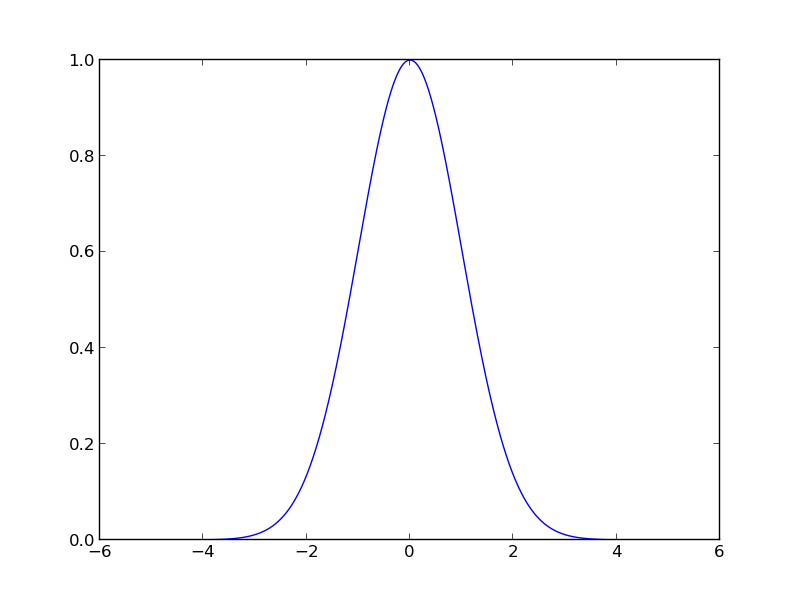
\includegraphics[width=1.0\linewidth]{images/gaussian.png}

    \end{columns}

\end{frame}


\begin{frame}[fragile]

    \frametitle{Gaussian Function}

\begin{lstlisting}
def gaussian(x):

    a = 1.0
    b = 0.0
    c = 1.0
    d = 0.0

    g = a*np.exp( -(x-b)**2 / (2*c**2) ) + d

    return g

\end{lstlisting}

\begin{lstlisting}
print gaussian(0.0)
\end{lstlisting}

\end{frame}


\begin{frame}[fragile]

    \frametitle{Gaussian Function}

    Multiple parameters

    \bigskip

\begin{lstlisting}
def gaussian(x, a):

    b = 0.0
    c = 1.0
    d = 0.0

    g = a*np.exp( -(x-b)**2 / (2*c**2) ) + d

    return g
\end{lstlisting}

\begin{lstlisting}
print gaussian(0.0, 1.0)
\end{lstlisting}

\end{frame}

\begin{frame}[fragile]
    \frametitle{15 min break}
    \begin{center}
        
\includegraphics[width=0.65\textwidth]{images/grumpy_cat.png}
    \end{center}
\end{frame}


\begin{frame}[fragile]

    \frametitle{files}

\begin{lstlisting}
f = open('filename', 'w')
f.write('line text')
\end{lstlisting}

\begin{lstlisting}
f = open('filename', 'r')
for line in file:
    print line
\end{lstlisting}

\end{frame}


\begin{frame}[fragile]

    \frametitle{Bifurcation diagram}

    http://en.wikipedia.org/wiki/Bifurcation\_diagram

    \bigskip

    \begin{equation*}
        x_{n+1} = x_n^2 - r
    \end{equation*}

    \bigskip

    Simulate the iterative process

    \begin{itemize}

        \item Simulate equation with initial guess $x=0.1$ and $r$ between 0.0 and 2.0 (hint: use \code{np.linspace}) and dump the data into a csv file
        \item Plot the csv data

    \end{itemize}

\end{frame}



\begin{frame}[fragile]

    \frametitle{Debugging}


    \begin{columns}[t]

        \column{0.4\linewidth}

            Typical errors:

            \begin{itemize}
                \item Indentation error
                \item Out of bounds
                \item Object not callable
                \item Invalid syntax
            \end{itemize}

        \column{0.5\linewidth}

        
            
\includegraphics[width=0.8\linewidth]{images/flip.jpg}

    \end{columns}


\end{frame}



\begin{frame}[fragile]

    \frametitle{Exercise Week 2 and program structure}

\begin{lstlisting}
import numpy as np
# ...
def initialize_particles(n_particles):
    """ Initialze particles positions and velocities """
    return positions_x, positions_y, velocities_x, velocities_y
# ...
n_particles = 40
# ...
pos_x, pos_y, vel_x, vel_y = initialze_particles(n_particles)

\end{lstlisting}

    \begin{itemize}
        \item import modules
        \item define functions
        \item define variables
        \item use functions with variables
    \end{itemize}

    \begin{itemize}
        \item Always keep functions in the beginning
        \item don't use global variables in functions
    \end{itemize}

\end{frame}




%%%%%%%%%%%%%%%%%%%%%%%%%%%%%%%%%%%%%%%%%%%%%%%%%%%%%%%%%%%%%%%%%%%%%%
%% END FRAMES
%%%%%%%%%%%%%%%%%%%%%%%%%%%%%%%%%%%%%%%%%%%%%%%%%%%%%%%%%%%%%%%%%%%%%%

\end{document}

